\subsection{Problem definition}

A slice with a hole in its centre, that means a 2D annulus, which consists of a solid of a constant temperature is exposed to a higher temperature at the surface of its hole. The aim of this calculation is to simulate the heat transfer through this homogeneous solid by the use of an axisymmetric model. Fig.~\ref{figT1} shows a sketch of the calculation area
\begin{figure}%[htbp]
\centering
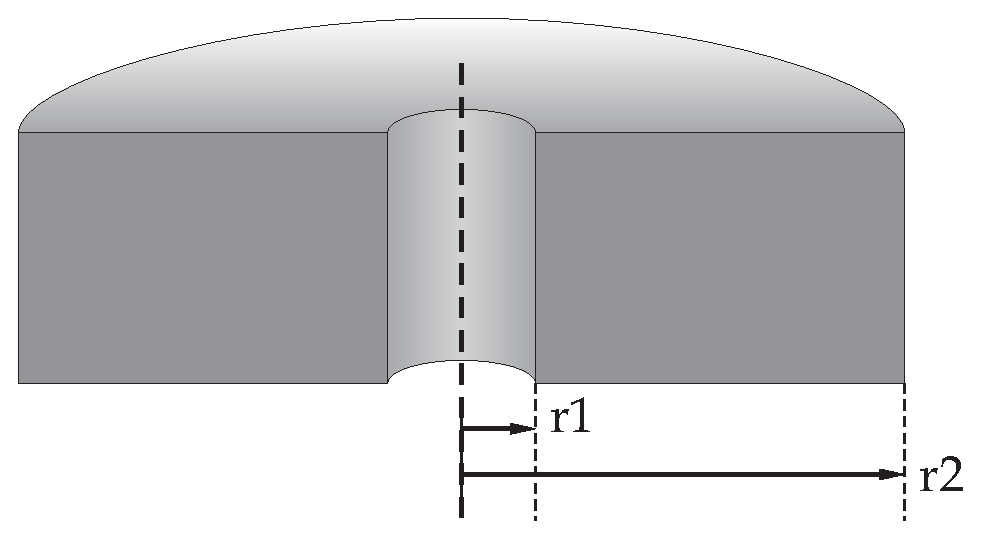
\includegraphics[width=0.5\textwidth]{T/figures/radial-heat-transport.eps}
\caption{\label{figT1}Calculation area.}
\end{figure}
assuming a homogeneous solid, a constant temperature in the whole body at the beginning and a heating of the slice at the inner surface of the hole .
%\textsl{Assumptions}
%
%\begin{tabbing}
%\=xxxxxxxxxxxxx  \=xxxxxxxxxxxxxxxxxxxxxxx \kill
%\> Temperature: \> constant temperature in the whole body at the beginning, \\
%\>  \> heating of the slice at the inner surface of the hole \\[0.5ex]
%\> Solid:		    \> homogeneous
%\end{tabbing}

\subsection{Model set-up of the 1D numerical model}

The inner radius $R_1$ of the axisymmetric model is $\unit[1]{m}$ and the outer radius $R_2$ is $\unit[5]{m}$. The numerical model consists of 40 elements and 41 nodes. The initial temperature in the whole area is $\unit[25]{^{\circ}C}$. At the right boundary of the numerical model a thermal boundary condition is set with a constant value of $\unit[25]{^{\circ}C}$. At the left boundary a source term for heat flux of $q=\unit[30]{W/m^2}$ is defined. Thereby the continuous heating of the solid is simulated. The used parameters of the solid are listed in Tab.~\ref{tab11}. The simulation of 5000 time steps with a constant time step length of $\unit[1000]{s}$ is done.
\begin{table}[h]
\caption{\label{tab11}Material properties.}
\begin{center}
\begin{tabular}{ll}
\toprule
parameter 						& value \\
\midrule
density of the solid $\rho$ 	& $\unit[2.0]{t \cdot m^{-3}}$ \\			
thermal capacity $c$		    & $\unit[900]{J \cdot kg^{-1} \cdot K^{-1}}$ \\
thermal conductivity $\lambda$	& $\unit[5.5]{W \cdot m^{-1} \cdot K^{-1}}$ \\
\bottomrule
\end{tabular}
\end{center}
\end{table}

\subsection{Evaluation method}

For the heating of the annulus with the inner radius $R_1$ and the outer radius $R_2$ the following analytical solution for temperature in dependency on the radius $r$ was used
\begin{equation}
T(r) = \frac{R_1 q}{\kappa}\ln\left(\frac{R_2}{r}\right) + T_0.
\label{eq11}
\end{equation}
Here $q$ represents the heat source, $\lambda$ the thermal conductivity and $T_0$ the initial temperature.
%{\small
%with
%\begin{itemize}
%\item[$q$] -- heat source (W/m$^2$)
%\item[$\lambda$] -- thermal conductivity (W/(m$\cdot$K))
%\item[$T_0$] -- initial temperature ($^{\circ}$C)
%\end{itemize}
%}

\subsection{Results}

The results of the analytical equation for the temperature distribution over the model length are compared to those of the numerical simulation by GeoSys/RockFlow. Fig.~\ref{figT2} shows the temperature distribution over the radius of the annulus. Obviously, with the axisymmetric model a GeoSys/RockFlow simulation generates comprehensible results that agree well with the analytic solution.
\begin{figure}[htbp]
\centering
\includegraphics[width=0.75\textwidth]{T/figures/figT2.eps}
\caption{\label{figT2}Temperature distribution over the radius}
\end{figure}

\begin{table}[h]
\caption{Benchmark deposit}
\begin{center}
\begin{tabular}{lll}
\toprule
Deposit & Version & Date \\
\midrule
T$\backslash$heat1d$\backslash$T\_1D\_axi & 4.7.02 & Mar.~2008 \\
\bottomrule
\end{tabular}
\end{center}
\end{table}
%\clearpage

